\documentclass[12pt]{article}
%\usepackage[utf8]{inputenc}
%\documentclass[UTF8]{ctexart}
%\usepackage[UTF8, heading = false, scheme = plain]{ctex}
\usepackage{geometry}
%geometry{a4paper,scale=0.9}
\geometry{a4paper,left=1cm,right=1cm,top=1cm,bottom=2cm}
\usepackage{amsfonts}
\usepackage{color}
\usepackage{url}
%\usepackage{biblatex}
\usepackage{amsmath}
\usepackage{amssymb}
\usepackage{latexsym}
\usepackage{cite}
%\addbibresource{ref.bib}
%\bibliography{ref.bib}
\usepackage{caption}
\usepackage{graphicx, subfig}
\usepackage{float}
%\usepackage[fontset=ubuntu]{ctex}
%\usepackage{fontspec}
\usepackage{xeCJK}
%\usepackage[colorlinks,
%anchorcolor=black,
%citecolor=black]{hyperref}
%\setmainfont{SimSun}
\usepackage[section]{placeins}
\usepackage{enumitem}
\usepackage{framed}
\usepackage[framemethod=TikZ]{mdframed}
\usepackage{indentfirst}
\usepackage{setspace}%使用间距宏包
\linespread{1.5}

\title{倾向性得分匹配介绍\cite{Talk_About_Causal_Inference_Part_2}}
\author{leolinuxer}
%\date{June 2020}

\begin{document}
%\setlength{\parindent}{0pt}
\maketitle
\tableofcontents

\section{倾向性得分匹配简介}
\begin{framed}
倾向评分匹配是一种统计学方法,用于处理观察研究的数据。

在观察研究中,由于种种原因,数据偏差和混杂变量较多。

倾向评分匹配的方法正是为了减少这些偏差和混杂变量的影响,以便对实验组和对照组进行更合理的比较。
\end{framed}

\section{因果推断数据集}
在介绍倾向性得分匹配之前,我们介绍一个观察性研究中非常经典的数据集:The NSW Dataset。

数据集分为两部分:
\begin{itemize}
\setlength{\itemsep}{0pt}
\setlength{\parsep}{0pt}
\setlength{\parskip}{0pt}
    \item 实验组:nswre74\_treated.txt (185 observations)
    \item 对照组:nswre74\_control.txt (260 observations)
\end{itemize}

在下文中,我们把随机实验数据称为 NSW-Data-Exp,把观察性研究数据称为 NSW-Data-Obs(“观察性研究” 数据的构造方式是取随机实验中的实验组,再搭配上一个通过其他渠道获得的对照组。)。我们先看看数据集里具体都有些什么。
\begin{itemize}
\setlength{\itemsep}{0pt}
\setlength{\parsep}{0pt}
\setlength{\parskip}{0pt}
    \item 样本属性 $X$: age, educ, black, hispan, married, nodegree (没有学位), re74(1974 年的收入), re75 (1975 年的收入)
    \item 干预 $T$: treat (是否接受了就业培训)
    \item 观察结果 $Y$: re78 (1978 年的收入)
\end{itemize}

下表是每一个数据集按照 treat 分组后的统计结果。
\begin{figure}[H]
    \centering
    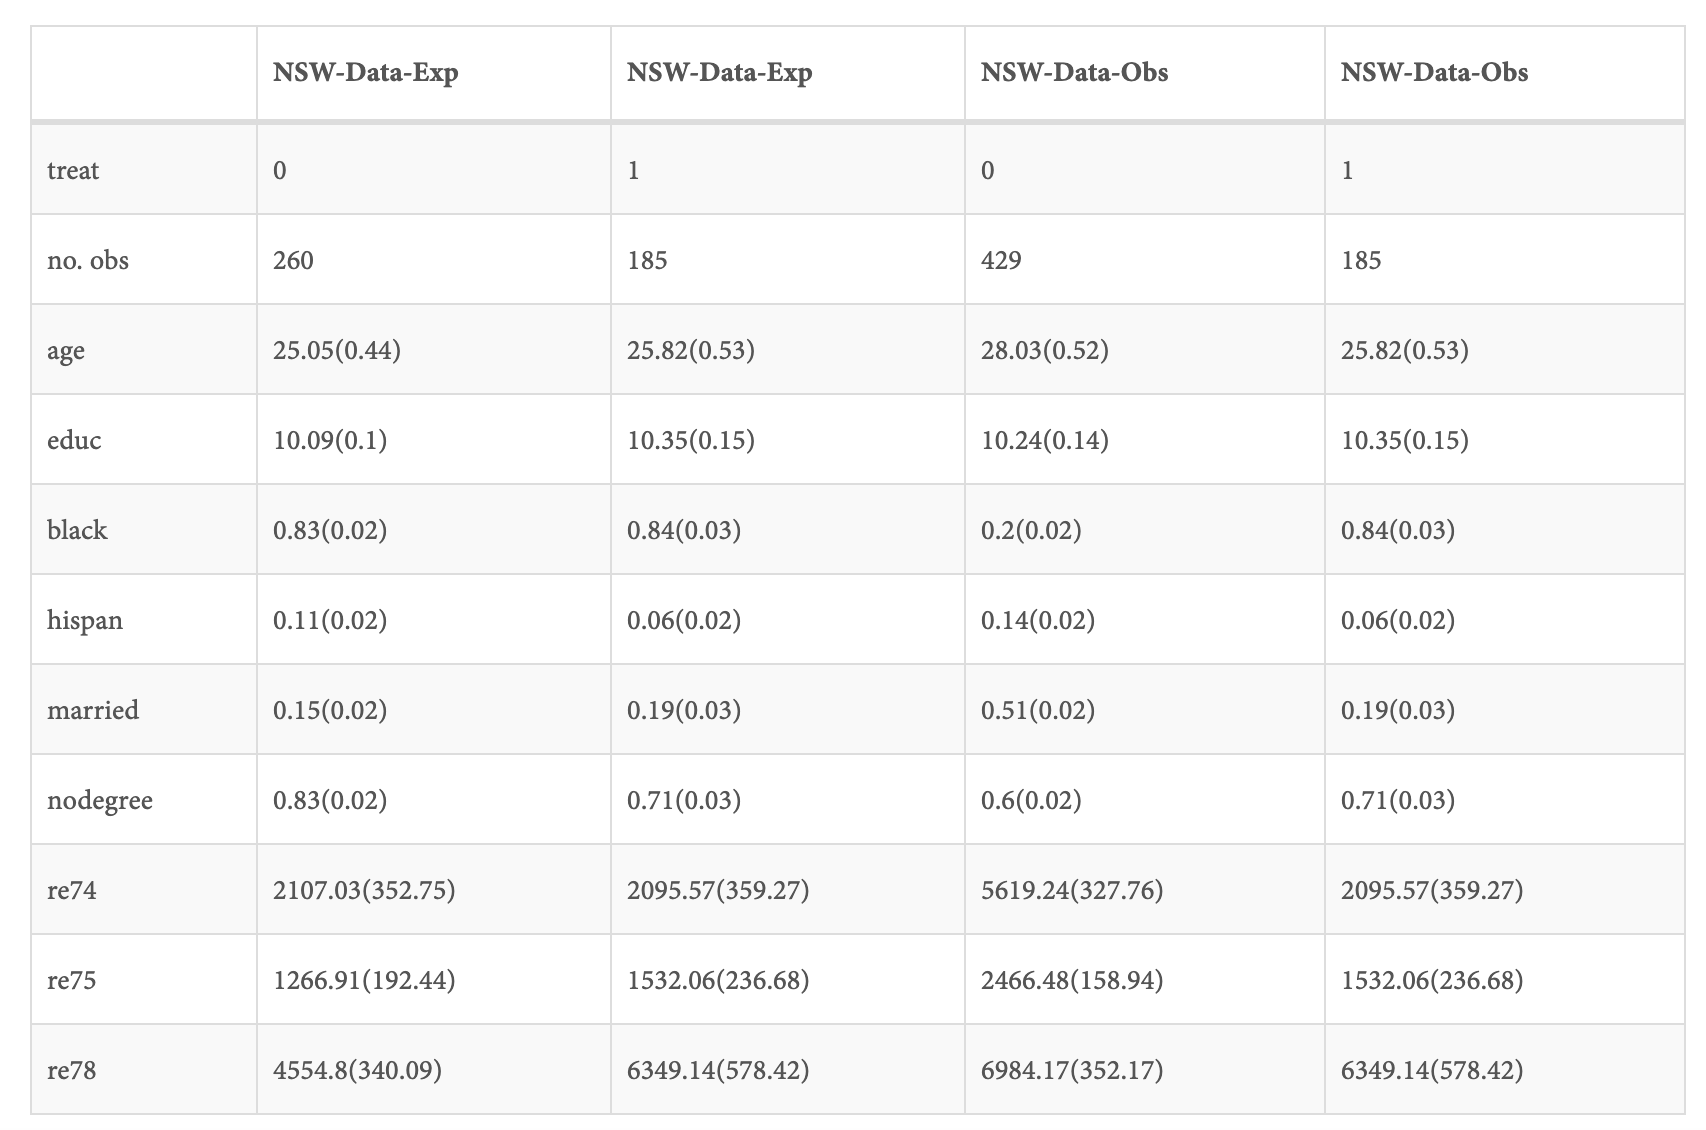
\includegraphics[width=1\textwidth]{fig/CasualInference-NSW-Data.png}
\end{figure}

随机实验数据 NSW-Data-Exp 中:实验组和对照组样本的各类属性都是很接近的,实验组 78 年的收入比对照组高 1794 美元,可以认为是就业培训带来的因果效应。

观察性研究数据 NSW-Data-Obs ()中: 实验后,实验组用户的收入比对照组低 635 美金,容易造成 “就业培训导致收入下降” 的幻觉,但是仔细一看,实验组用户在实验前的收入也比对照组低很多,所以两组用户实验后的收入本来就没有什么可比性。

在互联网公司里做数据分析时,日常数据分析工作里也常常遇到类似的问题:当我们想要分析一个产品特性、一个推荐策略、一个广告投放效果好不好时,我们的第一个尝试往往是把用户根据有没有命中或者有没有曝光 分成 “有” 和 “没有” 两组。

而在大部分时候,这两组用户是超级不同质的(例如被投放广告的用户可能是精挑细选的高潜力目标用户),所以比较起来也没有多大意义。

\section{倾向性得分匹配}
不论在 NSW-Data-Obs 这个数据集里,还是在上面提到的数据分析工作遇到的问题里,我们遇到的问题本质上\textbf{都是想要比较的两个人群不同质}。如果我们想要消除两个人群之间的不同质,让两个人群之间可以比较,我们可以怎么做呢?

一个粗暴的思路是将实验组和对照组的样本做一下 “匹配”。例如,对于实验组的每一个样本,我们都去对照组里找一个一模一样的样本。当样本属性全部都是离散的,并且属性的维度(个数)很小的时候,这么做也许是可以的。当样本属性里有一些连续变量或者当样本属性的维度很高时,这么做太粗暴了,大部分人是找不到匹配对象的。

“倾向性得分匹配”,简单而言,是一种更加靠谱的找对象方案。
在介绍 “倾向性得分匹配” 的过程中,我们也同步用经典的 NSW-Data-obs 做一份数据分析。

对于互联网公司的我,“样本” 和 “样本属性” 这些名词有一些距离感,下文里用 “用户” 和 “特征” 代替,加强一下代入感。

\subsection{倾向性得分的定义}
“倾向性得分” 的定义很直观,是一个用户属于实验组的 “倾向性”: 
$$
e(x) = Pr[X=1|X=x]
$$

倾向性得分是一种 “balancing score”。所有的 balancing score 都有两个很好的性质,可以总结为以下两个定理。如果感兴趣证明,可以参考 Imbens \& Rubin 的 Causal Inference 教科书 (Imbens G W, Rubin D B. Causal inference in statistics, social, and biomedical sciences[M]. Cambridge University Press, 2015.)第十二章。

\begin{mdframed}[
linecolor=black!40,outerlinewidth=1pt,roundcorner=.5em,innertopmargin=1ex,innerbottommargin=.5\baselineskip,innerrightmargin=1em,innerleftmargin=1em,backgroundcolor=gray!5,
%backgroundcolor=blue!10,%userdefinedwidth=1\textwidth,%shadow=true,%shadowsize=6,%shadowcolor=black!20,%frametitle={The \textit{two-step} model of XMCD:},%frametitlebackgroundcolor=cyan!40,%frametitlerulewidth=10pt
]
\begin{itemize}
\setlength{\itemsep}{0pt}
\setlength{\parsep}{0pt}
\setlength{\parskip}{0pt}
    \item \textbf{Theorem 1 (Balancing Property). $T_i \bot X_i|e(X_i)$}
    \item \textbf{Theorem 2 (Unconfoundedness). $T_i \bot Y_{i0},Y_{i1}|e(X_i)$}
\end{itemize}
\end{mdframed}

直观来说,对于倾向性得分相同的一群用户,treatment 和特征是独立的,treatment 和潜在结果也是独立的。
因此,理论上,如果我们对每一个实验组用户都在对照组里匹配一个得分相等(要求有点严苛)的用户,我们就能得到同质的实验组和对照组,就可以假装我们做了一个 A/B Test 了,接着就可以随意地进行组间比较了。

上面这段话具体实施起来,可以分为以下几个步骤。

\begin{itemize}
\setlength{\itemsep}{0pt}
\setlength{\parsep}{0pt}
\setlength{\parskip}{0pt}
    \item 倾向性得分估算:倾向性得分一般来说是未知的,怎么估算?         
    \item 倾向性得分匹配:怎么匹配?
    \item 平衡性检查:怎么量化匹配效果?
    \item 因果效应估算:怎么从匹配后的两组用户中得到因果效应?
    \item 敏感度分析:分析结论对于混淆变量选没选对(不满足 unconfoundedness )是不是很敏感?
\end{itemize}

\subsection{具体步骤}
\subsubsection{倾向性得分估算}
这一步说白了,就是一个建模问题。
一般来说,按需做一下特征预处理,然后套一下 LR 就可以了。
如果发现某些变量匹配效果不好(之后会介绍如何量化 “匹配效果”),可以考虑加入一些高阶项,从这一步重来一遍。

个人也试过使用 LR + LightGBM 估算倾向性得分,然后选 AUC 比较高的模型,在自己生成的仿真数据上看了一下,确实效果好一些。
但是关于倾向性得分估算到底要不要上复杂模型,其实是一个
trade-off,如果每次做分析都要做参数网格搜索甚至需要人肉调参,好像也不太实际对吧。

\subsubsection{倾向性得分匹配}
假设我们已经有了每个用户的倾向性得分,我们的目标是针对目前的实验组用户,匹配得到一个近乎于同质的对照组。

当用户量足够时候,一个简单做法是进行一对一无放回匹配:对于每一个实验组用户,我们去对照组里找一个倾向性得分最近的用户,把他们配成一对。匹配过程中,可以限制一下配对用户的得分差异不能超过某一个阈值,配不上就算了,以防把 “太不相似” 的用户匹配在一起。

在实现匹配时,有很多细节有很多选项,下面列一下个人认为比较常见的。和机器学习里调每个参数都对应着某些 trade-off 类似,这里每个选项背后也都有对应的 bias-variance 的 trade-off 的,就不细说。

\begin{itemize}
\setlength{\itemsep}{0pt}
\setlength{\parsep}{0pt}
\setlength{\parskip}{0pt}
    \item 匹配用的得分:可选原始倾向性得分 $e(x)$ 或者得分的logit
$l(x)=ln(e(x)/(1−e(x)))$,接下来都统一用 $e$ 表示。
        
    \item 修剪(trimming):秉承着 “希望下一个通用的结论” 的思路,可以先筛选掉倾向性得分比较 “极端” 的用户,例如在现实中不大可能出现在实验组里的对照组用户。常见的做法是保留得分在$[e_{min}, e_{max}] $这个区间的用户,关于区间选择,下面是两个例子。
    \begin{itemize}
\setlength{\itemsep}{0pt}
\setlength{\parsep}{0pt}
\setlength{\parskip}{0pt}
	\item 实验组和对照组用户得分区间的交集
	\item 只保留区间中部 90\% 或者 95\%,如取原始得分在 [0.05,0.95] 的用户
\end{itemize}

    \item 匹配(matching):实验组对对照组根据得分进行匹配时候,比较常见的有以下两种方法
        \begin{itemize}
\setlength{\itemsep}{0pt}
\setlength{\parsep}{0pt}
\setlength{\parskip}{0pt}
	\item nearest neighbors: 进行 1 对 K 有放回或无放回匹配
	\item radius: 对每个实验组用户,匹配上所有得分差异小于指定 radius 的用户
\end{itemize}

    \item 得分差异上限(caliper):当我们匹配用户的时候,我们要求每一对用户的得分差异不超过指定
的 caliper,“强扭的瓜不甜”,匹配不好就不要放弃吧。
\end{itemize}


\subsubsection{平衡性检查}
怎么衡量 “配平效果 “呢?

比较直观的是看倾向性得分在匹配前后的分布、以及特征在匹配前后的 QQ-Plot(??QQ-Plot是什么??)。

\subsubsection{因果效应推断}
我们的目标是推断 $ATT$(Average Treatment Effect on the Treated)。

回顾一下,$ATT$ 的定义为 $ATT=E[Y_1−Y_0|T=1]$。

现在我们已经有一对接近同质的实验组和对照组了,有很多方法可以用来估算 $ATT $。

个人感觉两种比较直观是:
\begin{itemize}
\setlength{\itemsep}{0pt}
\setlength{\parsep}{0pt}
\setlength{\parskip}{0pt}
	\item 直接比较匹配后的实验组和对照组
	\item 拟合一个由干预和用户特征预测观察结果的线形模型,看看干预 $T$ 的系数是多少
	\item ……
\end{itemize}

\subsubsection{敏感性检查}
敏感性分析的方法是独立于倾向性得分匹配的。

主要的目标是衡量当混淆变量(特征)不满足 unconfoundedness 时,分析结论是不是 robust。一个简单的做法是去掉一个或者多个混淆变量重复上面的过程,如果分析结论翻脸如翻书,说明
unconfoundedness 要么依赖于所有特征,要么不成立。

\section{扩展阅读}
关于倾向性得分匹配,有一篇引用超过 4000 的 Some practical guidance for the implementation of propensity score matching,感兴趣的小伙伴可以读一读。上面所写,只是其中的一个小小子集。

倾向性得分的其它打开方式:倾向性得分除了用来匹配,还有其它的用法。例如,我们可以用倾向性得分来对用户进行分组,称为 subclassification。我们还可以用倾向性得分来对用户进行加权,称为 Inverse Propensity Score Weighting (IPSW)。万变不离其中,目标都是为了消除两组用户的不同质导致的分析偏差。

%\printbibliography
\bibliography{../ref}
\bibliographystyle{IEEEtran}
\end{document}